\section{Literature}
Two-phase flow instabilities have been extensively studied for numerous industrial applications, including thermosiphons and power cycle loops.
Therefore, the literature of two-phase flow instabilities is extensive.
It should be noted that single phase instabilities do exist and are researched \cite{satoh_instability_1998}, but an in-depth overview of those mechanisms will not be given.
As such, an overview of two-phase instabilities, classifications, and definitions will be given.
Then, specific discussion of efforts and techniques in the analysis will be discussed.

\subsection{Two-Phase Flow Instabilities}
There are a variety of ways to classify two-phase flow instabilities depending on geometry, spatial/temporal dependence, multiphase models, etc.
Difficulties also arise when real world applications see a convergence of all of these parameters.
Both Boure \etal{} and Kakac \etal{} provide extensive discussions of general two-phase flow instability characterization \cite{boure_review_1973-1,kakac_review_2008-1}, and their similar systems for describing two-phase systems will be used throughout this section.
\Cref{Table:StaticInstabilities,Table:DynamicInstabilities} present a summary of general two-phase instabilities presented by the above authors; however, not all of them will be discussed in detail.
Presad \etal \cite{durga_prasad_review_2007-1} and Nayak \etal \cite{nayak_flow_2008-1}, while overlapping somewhat with the generic descriptions of instabilities, present and classify certain instabilities as natural circulation specific that should be described.
Most of the following discussion concerns a flowing fluid undergoing phase transition in a channel which may require some familiarity with two-phase flow regimes; explanation of these regimes is left to the literature \cite{thome_chapter_2004-1,tong_boiling_1997-1,ghiaasiaan_two-phase_2007-1}.


For clarity, key terms will be defined.
If a system at steady-state is perturbed and eventually returns to its initial equilibrium, the system is described as stable.
If a system at steady-state is perturbed into a neighborhood where no equilibrium exists near the initial state, the system possesses a static instability.
A system has dynamic instabilities if there are inherently transient feedback mechanisms that may lead to a steady-state, though there is no guarantee of uniqueness.
An instability that arises from another is referred to as a secondary phenomenon (the instigator being the primary).
\begin{figure}%
    \centering
    \caption[Ball-and-hill analogy of equilibrium descriptions]{
                Ball-and-hill analogy of equilibrium descriptions.  
                The ball represents some state at a given time and place, and 
                the shapes supporting the ball dictate how the state moves when subjected to a perturbation.
                Troughs are considered stable while crests/runoffs are unstable.}%
    \label{Figure:StabilityBAH}%
    %
    \vskip1em
    %
    \begin{subfigure}[t]{0.48\textwidth}%
        \centering
        \caption{Neutral equilibrium (infinitely many steady-states)}%
        \label{Figure:StabilityBAH:Neutral}
        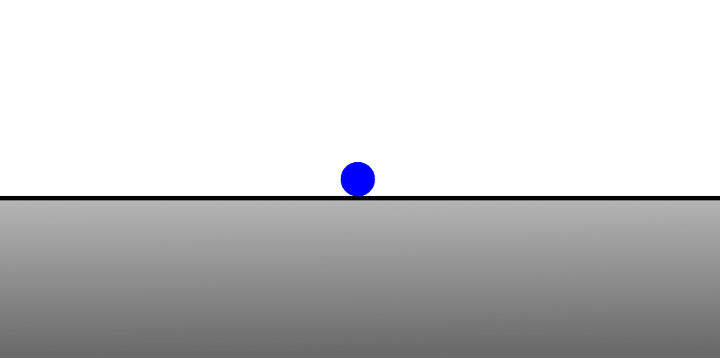
\includegraphics[width=0.85\textwidth]{NeutralEquilibirum.png}
    \end{subfigure}
    \hfill
    \begin{subfigure}[t]{0.48\textwidth}%
        \centering
        \caption{No equilibrium (no steady-state)}%
        \label{Figure:StabilityBAH:None}
        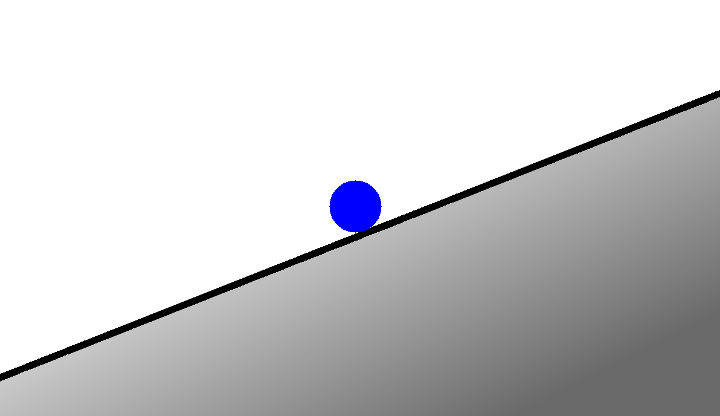
\includegraphics[width=0.85\textwidth]{NoEquilibirum.png}
    \end{subfigure}
    %
    \vskip3em
    %
    \begin{subfigure}[t]{0.48\textwidth}%
        \centering
        \caption[Stable equilibrium]{Stable equilibrium \vspace{1.5em}}%
        \label{Figure:StabilityBAH:Stable}
        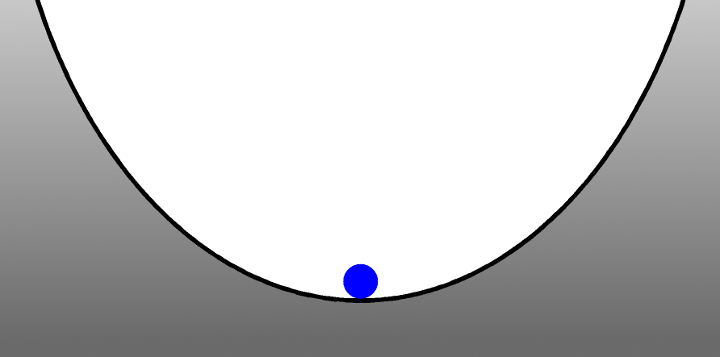
\includegraphics[width=0.85\textwidth]{Stable.png}
    \end{subfigure}
    \hfill
    \begin{subfigure}[t]{0.48\textwidth}%
        \centering
        \caption[Unstable equilibrium]{Unstable equilibrium \vspace{1.5em}}
        \label{Figure:StabilityBAH:Unstable}
        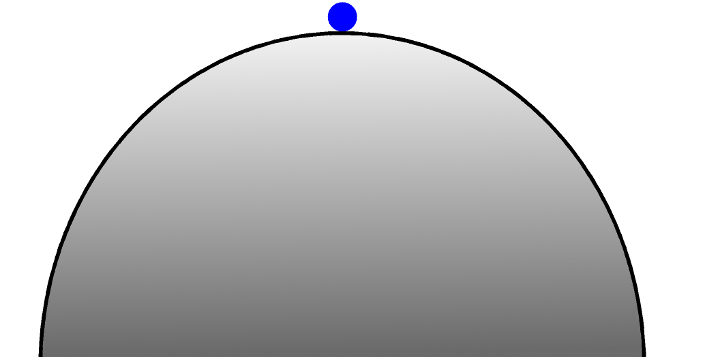
\includegraphics[width=0.85\textwidth]{Unstable.png}
    \end{subfigure}
    %
    \vskip3em
    %
    \newcommand{\LUNS}{Linearly unstable, nonlinearly stable equilibrium}
    \newcommand{\LSNU}{Linearly stable, nonlinearly unstable  equilibrium}
    \begin{subfigure}[t]{0.48\textwidth}%
        \centering
        \caption[\LUNS]{\LUNS\vspace{1.5em}}
        \label{Figure:StabilityBAH:LUNS}
        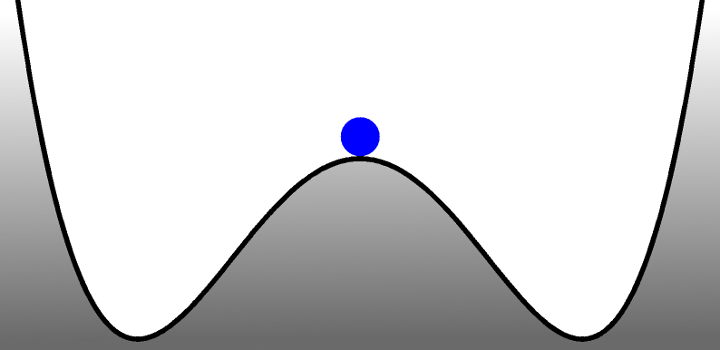
\includegraphics[width=0.85\textwidth]{LinearlyUnstableNonlinearlyStable.png}
    \end{subfigure}
    \hfill
    \begin{subfigure}[t]{0.48\textwidth}%
        \centering
        \caption[\LSNU]{\LSNU\vspace{1.5em}}
        \label{Figure:StabilityBAH:LSNU}
        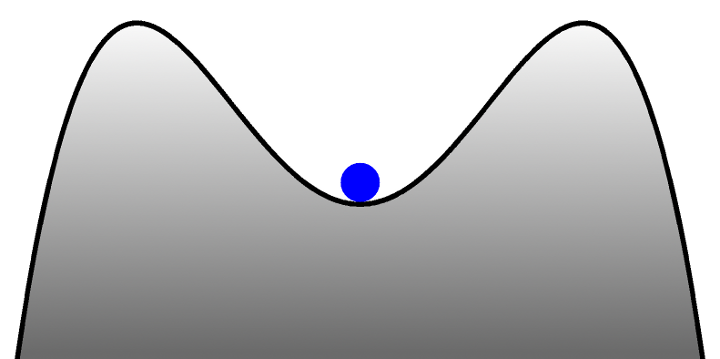
\includegraphics[width=0.85\textwidth]{LinearlyStableNonlinearlyUnstable.png}
    \end{subfigure}
\end{figure}
A compound instability is one that incorporates two or more mechanisms that confound analysis; fundamental instabilities are the opposite.  Using a standard physical analogy, \cref{Figure:StabilityBAH:Stable} is a stable system while \cref{Figure:StabilityBAH:Unstable} is an example of a system with a static instability.

One aspect of the stability the above definitions do not discuss is the magnitude of the system perturbations.
The strength of the perturbation is important since it determines how much energy is imparted into the system and, therefore, how far the system will travel from its initial state.
The importance can be seen in \cref{Figure:StabilityBAH:LUNS,Figure:StabilityBAH:LSNU} where both systems exhibit different behavior depending how hard the system is ``hit''.
\Cref{Figure:StabilityBAH:LUNS} shows a linear instability while actually being nonlinearly stable with multiple equilibria.
\Cref{Figure:StabilityBAH:LSNU} exhibits linear stability while being nonliearly stable
These concepts are important to consider when looking at linear stability because the behavior beyond the system's linear boundary is technically \textit{terra incognita}.
Actually performing a nonlinear analysis, if possible, is the only surefire tool for assessing stability.


\subsubsection{Static Instabilities}
Static instabilities are characterized by either a pure steady-state analysis or an analysis that foresees dynamic feedback from the steady-state system.
The analysis tools used to derive stability boundaries for these instabilities will be discussed in \cref{Section:StabilityTheory}.

A flow excursion, also known as a Ledinegg instability, is the sudden drop in a steady flow rate to a lower, steady value.
This jump occurs when the pressure losses in a system decrease with increasing flow rate.
For a liquid undergoing phase change in a channel, there is a complex, internal relationship between the buoyancy, friction, and acceleration momentum terms that must be taken into account for steady flow.
If the flow is forced by external sources and the internal forces of the flow are not properly taken into account, then the pressure drop could rise with increasing flow; this is especially true for slightly sub-cooled flows entering a heated region where a sudden change in void fraction can have a large impact on the flow behavior with the system.

Fundamental relaxation instabilities occur when two or more flow regimes have state equilibriums close to each other.
For example, a bubbly flow that experiences a small change in flow rate could transition to the annular regime.
Then, the flow rate will experience an increase since annular flow has a relatively low pressure drop, and the flow regime transitions back to the bubbly regime.
Given the right situation, this cycle could continue ad infinitum.
The flow regime transitions act as a relaxation mechanism (in the dynamical system sense) that causes persistent, periodic behavior.

Chugging is an instability associated with the jetting of large vapor structures from a flow channel into larger space.
This instability typically occurs with low velocities and moderate void fractions \cite{tong_boiling_1997-1}.
A flowing liquid receiving heat may develop large vapor bubbles in a coolant channel; this increases the flow rate due to the vapor-to-liquid ratio.
After the bubbles have been expelled, or possibly quenched, at the channel exit, the flow rate will return to the pre-slug rate.
As with the relaxation instability, this mechanism also has a periodic nature \cite{aritomi_geysering_1993-1}.



\subsubsection{Dynamic Instabilities}
Dynamic instabilities, unlike static, are inherently transient and primarily involve the transmission of information via waves.
\THs systems typically possess a material (density) wave and an acoustic (pressure) wave.
For a non-ideal fluid, the acoustic wave's speed is primarily a function of the system's density and temperature while the material wave travels near the physical speed of the system.

Acoustic instabilities are typically of high frequency ($10$Hz--$10$kHz) and have been observed in various boiling regimes.
The acoustic waves were found to cause large pressure drop oscillations relative to steady-state values.
Even in situations where the lower frequency density waves were present, there was a clear superposition of high frequency acoustic waves with the material waves.
At high pressure-and-temperature water experiments, the acoustic waves reached frequencies that were clearly audible (so-called whistler modes).

Material wave instabilities are the most common in two-phase flow and are a highly physical phenomenon that occur from a complex coupling of \THs equations, constitutive relations, and geometry.
These waves have also been described as ``flow-void feedback instabilities'' for boiling systems \cite{neal_mechanisms_1967-1} and ``time-delay oscillations'' due to the relatively slow transmission of information at material speed \cite{boure_oscillatory_1966-1}.
Since the oscillation has its roots in the differing densities of a fluid's liquid and gas phases, vertical channel height (where the system pressure changes greatly with position), inlet conditions (thermodynamic and kinematic), and total heat transfer between the fluid and the surroundings are extremely important in the control and appearance of these flow oscillations.
It has been found that by increasing the system pressure these oscillations can be mitigated or eliminated since the density ratio of the competing phases approach one another as the pressure increases.

These material oscillations can lead to oscillations in the boiling heat transfer processes at the wall and results in a compound thermal instability.
The emphasis here is put on the highly variable nature of the two-phase heat transfer coefficient at the wall and how the information being propagated from the wall interacts with material wave oscillations.
The effects of this interaction can be as bad as an oscillating dry point in the channel with large temperature oscillations.



\subsubsection{Natural Circulation Instabilities}
There are two natural circulation instabilities of primary interest: flashing and compound natural circulation.
As mentioned in \cref{Section:RCCS}, flashing occurs when a high temperature liquid flows into a region of lower pressure such that it enters a saturated or superheated state and immediately bursts into a two-phase mixture.
This mechanism is a primary cause of material wave instabilities in natural circulation loops at low pressures or long vertical channels.
This type of instability is currently under examination for one and two protypic fuel channels \cite{marcel_experimental_2009-1,marcel_experimental_2010-1}.

The final instability is the compound natural circulation instability.
This instability is the confluence of vertical channel heating, material wave oscillations (possibly due to flashing), chugging phenomenon, and flow regime transitions.
Since the system's flow rate is not subject to any mechanical head contributions, all of these instabilities can occur concurrently and must be carefully analyzed to discern which of the mechanisms are present and which is dominant.
These instabilities are extremely important for all types of nuclear reactors and are under continuously under investigation \cite{dauria_characterization_1990-1,aritomi_fundamental_1992-1,yun_two-phase_2005-1}.

\begin{table}
    \centering
    \caption[Summary of static flow instabilities]{Summary of static flow instabilities due to \cite{boure_review_1973-1}}
    \label{Table:StaticInstabilities}
    \rowcolors{2}{}{Gray}
    \setstretch{1.05}
    \renewcommand{\arraystretch}{1.4}
    {\small
    \hyphenation{Transition}
    \hyphenation{Relaxation}
    \begin{tabular}{>{\centering}p{1.15in} >{\centering}p{1.1in}  >{\raggedright}p{1.4in}  >{\raggedright\arraybackslash}p{1.5in} }
        \toprule
        \multicolumn{1}{c}{\textbf{Name}}      & \multicolumn{1}{c}{\textbf{Class}} & 
        \multicolumn{1}{c}{\textbf{Mechanism}} & \multicolumn{1}{c}{\textbf{Characteristics}}\\\midrule
        % --------------------------------------------------------------------------------- 
        Flow excursion                     & Fundamental            & 
                \LedineggCriterion & Sudden, large flow change to a new, stable state \\
        % ---------------------------------------------------------------------------------
        Boiling crisis                     & Fundamental            & 
                Ineffective cooling & Wall temperature excursion and flow oscillation \\
        % ---------------------------------------------------------------------------------
        Flow Regime  Transition             & Fundamental Relaxation & 
                Varying $\Delta{P}$ between regimes            & Cyclic flow pattern transitions and flow rate variations \\
        % ---------------------------------------------------------------------------------
        Bumping, geysering, or    chugging & Compound    Relaxation & 
                Periodic adjustment of metastable conditions & Periodic superheat and violent evaporation \\
    \bottomrule
    \end{tabular}
    }
\end{table}
\begin{table}
    \centering
    \caption[Summary of dynamic flow instabilities]{Summary of dynamic flow instabilities due to \cite{boure_review_1973-1}}
    \label{Table:DynamicInstabilities}
    \rowcolors{2}{}{Gray}
    \setstretch{1.05}
    \renewcommand{\arraystretch}{1.4}
    {\small
    \hyphenation{Compount}
    \hyphenation{Relaxation}
    \begin{tabular}{>{\centering}p{1.1in} >{\centering}p{1.1in} >{\raggedright}p{1.55in} >{\raggedright\arraybackslash}p{1.55in} }
        \toprule
        \multicolumn{1}{c}{\textbf{Name}}      & \multicolumn{1}{c}{\textbf{Class}} & 
        \multicolumn{1}{c}{\textbf{Mechanism}} & \multicolumn{1}{c}{\textbf{Characteristics}}\\\midrule
        % --------------------------------------------------------------------------------- 
        Acoustic  Oscillations  & Fundamental & Resonance of pressure waves & 
                High frequency oscillations near the acoustic speeds\\
        % ---------------------------------------------------------------------------------
        Density Wave  Oscillations  & Fundamental & Coupled mass, momentum, and energy feedback & 
                Low frequency oscillations near the material speed\\
        % ---------------------------------------------------------------------------------
        Thermal  Oscillations  & Compound & Variable heat transfer coefficient interacting with flow & 
                Occurs during film boiling \\
        % ---------------------------------------------------------------------------------
        BWR  Instability &  Compound & Hydraulic-neutronic coupling & 
                Strong only for a small fuel time constant and low pressure\\
        % ---------------------------------------------------------------------------------
        Parallel  Channel  Instability & Compound & Interaction among parallel channels & 
                Various modes of flow redistribution\\
        % ---------------------------------------------------------------------------------
        Pressure drop  Oscillations & Secondary Compound& 
                Flow excursions initiate interactions between channels and compressible volumes & 
                        Very low frequency, periodic process\\
    \bottomrule
    \end{tabular}
    }
\end{table}
\begin{table}
    \centering
    \caption[Effects of parametric variation on instability]
            {Effects of parametric variation on instability for a flow entering a vertical channel sub-cooled or saturated 
             due to \cite{durga_prasad_review_2007-1}}
    \label{Table:ParametericEffects}
    \rowcolors{2}{}{Gray}
    \setstretch{1.05}
    \renewcommand{\arraystretch}{1.5}
    {\small
    \hyphenation{Transition}
    \hyphenation{Relaxation}
    \begin{tabular}{>{\centering}p{1.6in} >{\raggedright}p{1.3in} >{\raggedright\arraybackslash}p{2.8in}}
        \toprule
        \multicolumn{1}{c}{\textbf{Parameter Increased}}  & \multicolumn{1}{c}{\textbf{Effect}} & 
        \multicolumn{1}{c}{\textbf{Reason}}\\\midrule
        % --------------------------------------------------------------------------------- 
        System pressure & Stability increases & Phase density difference lessens thus reducing the gravitational head gain. \\
        % ---------------------------------------------------------------------------------
        Mass flow rate  & Stability increases & Critical power for oscillation generation increases and avoids chugging.\\
        % ---------------------------------------------------------------------------------
        Inlet sub-cooling& Destabilizes at small sub-coolings but stabilizes otherwise &
                For small sub-coolings,due to significant response delay in void formation with an increase in transit time.
                Otherwise, it reduces void fraction and increases non-boiling length.\\
        % ---------------------------------------------------------------------------------
        Inlet resistance & Stability increases & Increases the single phase friction which has a damping effect upstream.\\
        % ---------------------------------------------------------------------------------
        Exist resistance & Stability reduces   & Increases two-phase friction which amplifies instabilities upstream\\
        % ---------------------------------------------------------------------------------
        Riser height     & Stability reduces   & 
                Increases two-phase gravitational pressure drop and phase transition as static head decreases\\
    \bottomrule
    \end{tabular}
    }
\end{table}


\newpage
\subsection{Previous Analysis Efforts}
The two main types of analysis employed in stability analysis are linear and nonlinear (nonlinear being a superset of the other).
Every analysis begins with a defined set of the conservation/balance equations.
These equations possess all of the modeling information and assumptions in the analysis to be performed.
Three commonly used models are \cite{johnson_handbook_1998}:
\begin{itemize}
    \item{a homogeneous equilibrium model (HEM) where the distinct phases of a boiling fluid are treated as a single fluid with averaged properties;}
    \item{a separated flow model (SFM) where an additional momentum equation is added to the HEM allowing phase slip;}
    \item{a two-fluid model where the distinct phases are treated as separate partitions of a total volume, have completely separate properties, and only communicate through their shared interface.}
\end{itemize}
\Cref{Chapter:Theory} discusses the HEM and two-fluid equations, but for now, it suffices to say that these equations are nonlinear, coupled partial differentials equations that do not, in general, admit analytical solutions.

After the model has been decided, authors either linearize the equations or not and assess the system's stability through various techniques.
The specifics of the solution techniques are left to \cref{Section:StabilityTheory} since the techniques are all similar.
What makes the approaches more interesting is the models used, approximations made, and geometry considered.

Wallis and Heasley present one of the earliest efforts to analytically tackle two-phase flow oscillations \cite{wallis_oscillations_1961}.
They investigated a simple, closed natural circulation loop with pentane as the working fluid.
The analysis method looked at three sources of oscillations from a Lagrangian frame.
The first source was changes in riser buoyancy resulting from velocity perturbations and an equation for the marginal stability was derived in terms of the friction factor's derivative with respect to some steady-state velocity.
The second source was the heat input into the system with a theorized flow excursion for their loop.
Lastly, they investigated parallel channels but did not complete the analysis due to the then intractability of the solution.

Welander, though not a study of two-phase instabilities, investigates a simple, closed loop with point sources and proportional constitutive relations.\cite{welander_oscillatory_1967}.
While the treatment is similar to Wallis and Heasley's, Welander's more mathematical approach is more in-line with this work's goals.
Additionally, Welander derived an asymptotic steady-state solution and also compared the analytical neutral boundary with numerical experiments to confirm the boundary's validity.
Zvirin and Greif continued this work by examining how an arbitrary initial condition evolved toward Welander's steady state \cite{zvirin_transient_1979}.
They found that while the solution approached the analytical steady-state, the solution was without oscillation and concluded that the oscillation characteristics were strongly dependent on the shape of the initial condition.

Achard \etal investigated material wave oscillations in a horizontal boiling channel using both linear and nonlinear analysis \cite{achard_analysis_1985}.
They derived a lumped parameter integrodifferential equation.
Upon linearizing the equation and using the friction and sub-cooling numbers as degrees of freedom, they found two absolutely unstable regions, several conditionally unstable regions, and one absolutely stable region.
The conditionally unstable regions were found to depend on how actual system's state evolved in time and moved through the stability space.
They also performed a nonlinear analysis where the parameter values to maintain stability were obtained by nonlinearly solving the lumped parameter equation for a given perturbation amplitude.
The nonlinear analysis showed that stable parameter curves existed for their system but the absolutely stable region shrank with increasing perturbation amplitude.

Lee and Ishii performed a linear analysis similar to Welander, but the system was explicitly two-phase, had a quadratic frictional dependence in velocity with a constant friction factor, and had a distributed heat load \cite{sang_yong_lee_thermally_1990}.
Additionally, as an extension of the Zvirin and Greif's methodology, Lee and Ishii divided the loop into size different regions with average properties and solved for the stability boundary using linear analysis.

Lee and Lee performed nearly the same analysis as Lee and Ishii with the added difficulty of a variable, flow-regime dependent friction factor \cite{lee_linear_1991}.
Guanghui \etal also performed a similar analysis over a simple, closed loop that compared very well experiments \cite{guanghui_theoretical_2002}.

Knaani and Zvirin investigated the existence of multiple steady-states for a simple, closed loop undergoing boiling\cite{knaani_bifurcation_1993}.
The analysis was done with HEM and incorporated a guess and check procedure for finding a solution to the nonlinear problem.
They ultimately found multiple steady-states for the closed system due to the non-monotonic nature of the buoyancy term during phase change.
Nayak \etal also performed analysis on a simple, closed loop but used a four equation model (two for mass and mixture equations for energy and momentum) and several different two-phase friction multipliers \cite{nayak_study_2007}.

Lee and Pan undertook an \Acronym{HEM} for a two-phase natural circulation system with two parallel, heated channels \cite{lee_nonlinear_2005}.
This treatment is the first work in this review to explicitly analyze a non-simple closed loop.
Through a number of piece-wise integrations along the loop, the authors arrived at a set of ordinary differential equations that satisfied the zero pressure gradient requirement of the closed loop.
Using the channel inlet sub-cooling as a parametric and a blackbox solver, the authors compared the steady-state channel flow rates with experimental data.
The authors then found a stability curve for even heating of the channels that possessed two unstable regions and one stable region.
The author concluded with a parametric study of how the stability region shifted with the addition of an orifice plate.







